%%%%%%%%%%%%%%%%%%%%%%%%%%%%%%%%%%%%%%%%%%%%%%%%%%%%%%%%%%%%%%%%%%%%%%%%%%%%%%%%%%
\begin{frame}[fragile]\frametitle{}
\begin{center}
{\Large Deep Q Learning}
\end{center}
\end{frame}

%%%%%%%%%%%%%%%%%%%%%%%%%%%%%%%%%%%%%%%%%%%%%%%%%%%%%%%%%%%%%%%%%%%%%%%%%%%%%%%%%%
\begin{frame}[fragile]\frametitle{Problems with Q Learning}


\begin{itemize}
\item Q Learning is suitable for small states space, tabular methods
\item Inefficient for Large and continuous state space problems.
\item Not enough time, resources.
\item Deep Learning comes to rescue here.
\item Neural Networks can be Universal Function approximator. Can model continuous function as well.
\end{itemize}

{\tiny (Ref: Modern Reinforcement Learning: Deep Q Learning in PyTorch - Phil Tabor)}

\end{frame}

%%%%%%%%%%%%%%%%%%%%%%%%%%%%%%%%%%%%%%%%%%%%%%%%%%%%%%%%%%%%%%%%%%%%%%%%%%%%%%%%%%
\begin{frame}[fragile]\frametitle{Deep Learning}


\begin{itemize}
\item Can approximate any function-relationship
\item Being primarily Matrix Multiplications, can leverage GPUs
\item Each perceptron is linear combination of inputs times weights plus bias.
\item Non linearity is added to it via Activation functions like Relu and Sigmoid.
\end{itemize}

{\tiny (Ref: Modern Reinforcement Learning: Deep Q Learning in PyTorch - Phil Tabor)}

\begin{center}
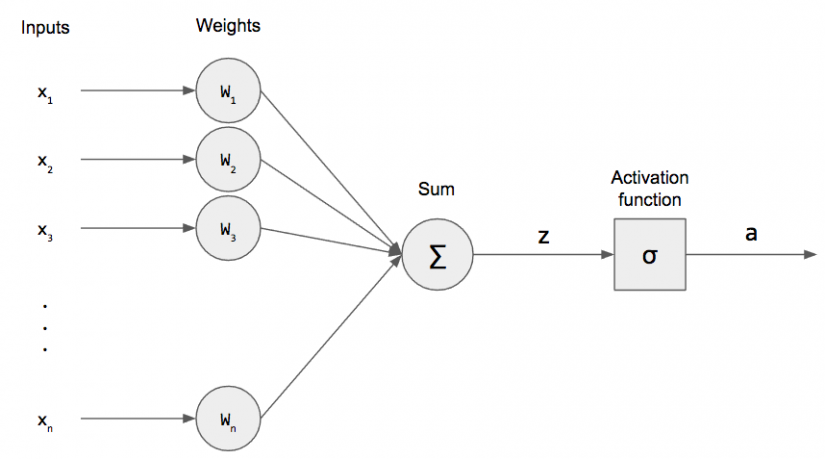
\includegraphics[width=0.6\linewidth,keepaspectratio]{rl69}

{\tiny (Ref: Python Machine Learning - Zenva)}
\end{center}

\end{frame}

%%%%%%%%%%%%%%%%%%%%%%%%%%%%%%%%%%%%%%%%%%%%%%%%%%%%%%%%%%%%%%%%%%%%%%%%%%%%%%%%%
\begin{frame}[fragile]\frametitle{Deep Learning Process}


\begin{itemize}
\item Input is fed into a layer and activated 
\item Result is then fed into next layer, and activated 
\item All the way through to the output
\item Output compared to some target to get cost 
\item  Weights changed to minimize cost (back propagation)
\item Repeat process $\rightarrow$ profit
\end{itemize}

{\tiny (Ref: Modern Reinforcement Learning: Deep Q Learning in PyTorch - Phil Tabor)}

\end{frame}

%%%%%%%%%%%%%%%%%%%%%%%%%%%%%%%%%%%%%%%%%%%%%%%%%%%%%%%%%%%%%%%%%%%%%%%%%%%%%%%%%
\begin{frame}[fragile]\frametitle{Deep Learning for Q Learning}


\begin{itemize}
\item Almost same structure as any standard but with MSE loss, Relu activation and a state-action-reward based Cost function
\item Inputs: states
\item Labels: actions
\item How it was made a supervised like learning problem? when there is no prior labeled data?
\item Target is $r + \gamma max Q(s',a_{max})$
\end{itemize}

{\tiny (Ref: Modern Reinforcement Learning: Deep Q Learning in PyTorch - Phil Tabor)}

\end{frame}